% !TEX root = ../../main.tex


\begin{figure}[tb]
{\small\texthv{\textbf{\,(a) True IBD}}} \\
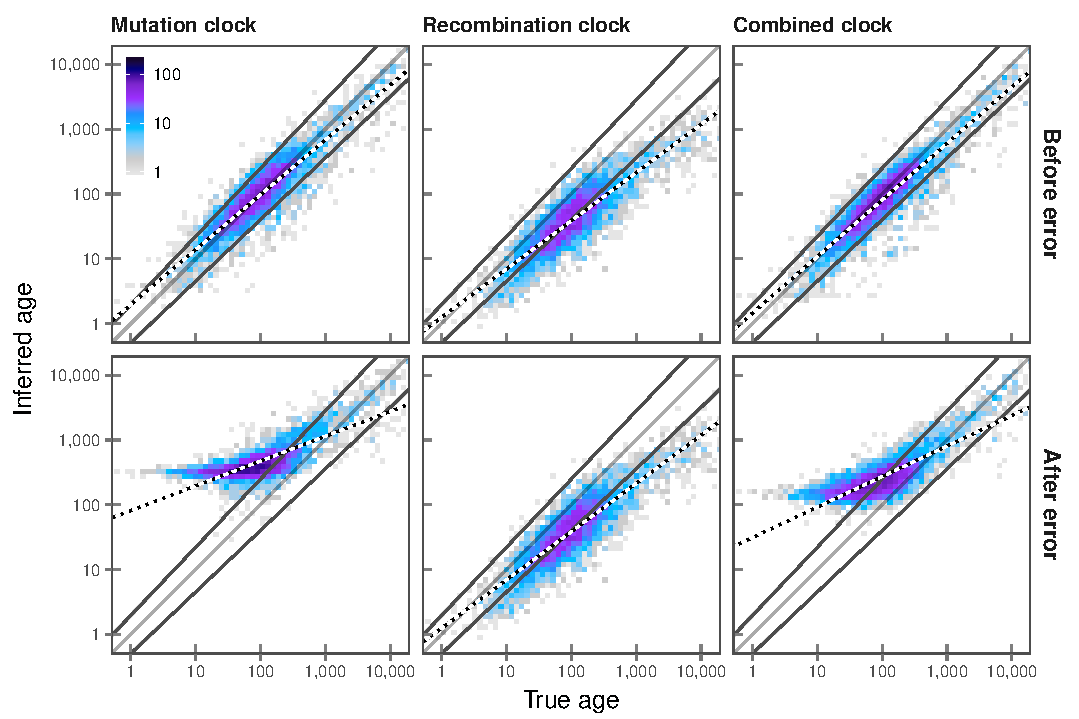
\includegraphics[width=\textwidth]{./img/ch5/generror_scat_tru}
\Caption{Density of allele age before and after error in simulated data}
{The effects on the estimation process \emph{before} and \emph{after} error are compared.
\Correct{Note that the ``true age'' was set to $t_m$, which is the geometric mean of $t_c$ and $t_d$.}
Lines \emph{below} and \emph{above} the dividing line correspond to the regression lines over $t_c$ and $t_d$; \ie of the times of coalescent events delimiting the branch on which a focual mutation occurred.
The \emph{black-white} line gives the regression for the inferred age ($\hat{t}$).
This panel (\textbf{a}) compares the distributions of true and inferred ages, which were estimated on basis of the true IBD structure of the sample as determined from simulation records.
The other panels show estimation results based on the different IBD detection methods;
\gls{fgt} on both true and phased haplotypes (\textbf{b}, \textbf{c}; \pref{fig:generror_scat_fgt}),
\gls{dgt} (\textbf{d}; \pref{fig:generror_scat_dgt}),
and the \Correct{genotype-based} \gls{hmm} (\textbf{e}; \pref{fig:generror_scat_hmm}).
Each analysis was conducted on the same set of \n{5000} randomly selected target variants at \fk{[2,25]}.}
{fig:generror_scat_tru}
\end{figure}
